\section{Methods for Measuring IPv6 Deployment}

\subsection{Prefix Allocation Data}

IPv6 addresses used across the internet are assigned by a hierarchy of
organisations;
the Internet Assigned Numbers Authority (IANA) having authoritative control of the
allocation of IPv6 addresses, and delegating the allocation of blocks of IPv6
addresses to the five Regional Internet Registries (RIRs) such as Réseaux IP Européens
Network Coordination Centre (RIPE NCC) which is the RIR for Europe. The RIRs administer the
address space in their region and are responsible for
allocating addresses to the Local Internet Registries (LIRs). The term prefix
refers to to the portion of the IPv6 network prefix (the first 64 bits of an
IPv6 address) that identifies a given block of addresses, and generally also
includes a prefix length. For example \verb+2001:630:d0::/48+ is the IPv6 prefix held by the
University of Southampton.

RIPE NCC keep records of and maintain statistics about all of the IPv6 addresses
allocated since 1999, which can be used as a metric for how IPv6 is being
deployed, either by counting the number of addresses allocated or by counting
the number of prefixes allocated (recording the number of requests made rather
than the size of subnets asked for). The other RIRs also maintain publicly
available records of their IPv6 and IPv4 prefix allocations, used by Geoff
Huston to generate and maintain historical
reports of IPv6 allocation worldwide, dated from mid-2006 to
present day\cite{huston_ipv6_2013}.

Analysis of this data has been performed by a number of sources. Kuhne tracks
the number of IPv6 allocations starting from 1999 until 2010 and identifies three
phases in the allocations of and hence requests made for IPv6 prefixes since
RIPE started allocating IPv6 addresses\cite{kuhne_interesting_2010}.
The first phase is identified between 1999 and
2002 as "experimental" where IPv6 and the mechanisms to support it were still
under development. The second phase identified between 2002 and 2007 showed
steady but low rates of adoption, that Kuhne contributes to early adopters. The
third phase identified from 2007 to the publication of the data in 2010 showed
an accelerating allocation rate, contributed to the increased efforts of RIRs
to promote IPv6 in light of the approach of the exhaustion of the IPv4 address
space. The three phases can be seen on the up to date graph of IPv6 allocations
by month from RIPE shown in Figure \ref{fig:alloc-month}. Karpilovsky et al. make
similar conclusions on the allocation data, despite not recognising the
experimental phase, Karpilovsky finds that number of allocations was linear
until 2008 when the rate of allocation significantly increased\cite{karpilovsky_quantifying_2009}.
Karpilovsky et
al. also attempt some analysis of the number of IPv6 address allocated over
time, but find that it is not possible to draw meaningful conclusions from this
data as it is dominated by a very small number of very large allocations.

\begin{figure}[htb]
\centering
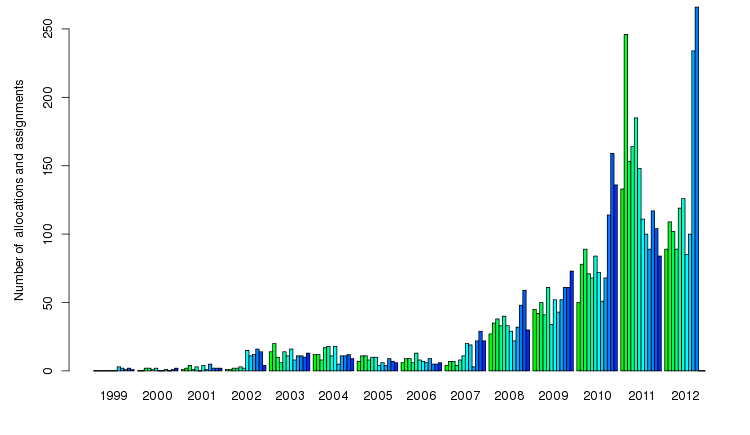
\includegraphics[width=0.4\textwidth]{img/v6-alloc-month.png}
\caption{IPv6 Prefix Allocations by RIPE per month (source \protect\cite{ripe_ncc_ipv6_2013})}
\label{fig:alloc-month}
\end{figure}

Another factor that may contribute to how the allocation of IPv6 prefixes is
affecting the deployment of IPv6 are the policies surrounding Provider Independent
(PI) addresses. In IPv6 most unicast addresses are globally aggregatable, to simplify the BGP
routing tables and ensure that the protocol can remain scalable despite the
vastly increased address space. These globally aggregatable addresses are
assigned to end users by their providers, but many organisations want to use an
address block that will not change if the organisation changes internet
provider, or want to increase network reliability by having a second link to the
internet that advertises the same address space. PI address space is a solution
to both of these issues, as address space is allocated directly from an LIR or
RIR, but is criticised for increasing the IPv6 routing tables in manner that may
not be scalable\cite{karrenberg_pi_1995}. Kuhne finds that following the relaxation of requirements
regarding PI allocation from RIPE NCC in February 2012, there was a dramatic increase in the 
number of PI allocations and hence overall IPv6 prefix allocations\cite{mirjam_kuhne_update_2012}.

The use of RIR allocation data as a metric for the deployment of IPv6 at first
seems to be fairly robust, but there are some caveats that must be considered.
Firstly, allocation does not equate to use, so we must turn to other sources of
data to qualify whether the addresses allocated are actually being used. Another
possible issue is that the allocation data published by the RIRs is generally
for allocation to LIRs, so allocation of prefixes to end users is not shown.

%TODO: - haven't looked at Geoff Huston's reports here.

\subsection{BGP Route Data}

Routing of traffic between the individual networks, known as Autonomous
Systems (ASs), that make up the Internet is performed using the Border Gateway
Protocol (BGP). Each BGP router on the Internet holds routing tables that
describe paths to every reachable AS on the internet (although ASs with
consecutive address space may be aggregated together).
Each AS announces its existence at the edge of its network, and this
information is propagated across the Internet.
The information held in the routing tables can be used to gain some measure of
the deployment of IPv6, as the routing tables provide an effective summary of
all reachable IPv6 prefixes. This data should give a better indication of IPv6
deployment than just the prefixes allocated\cite{karpilovsky_quantifying_2009}, as an AS must
have deployed some IPv6 infrastructure to advertise a network.

BGP routing data has been made publicly available by a number of sources, most
notably the routeviews\cite{meyer_route_2005} project hosted by the University of Oregon in the
US, and the Routing Information Service (RIS) project maintained by RIPE
NCC\cite{ripe_ncc_routing_????}.
Each of these projects offer live views of BGP routing data from various points
around the world, with routeviews retrieving data from 7 IPv6 enabled Internet
Exchange Points (IXPs) and the hosting University's own connection, whilst RIS
collects data from 13 IXPs and the RIPE NCC headquarters in Amsterdam. This data
is collected by deploying routers to these locations that peer with the other
IPv6 ASs that advertise routes there. Both RIS and routeviews keep historical data, with RIS
archiving data since 1999 (although this does not necessarily contain IPv6 data
from this time) and routeviews archiving data since 2001. 
%TODO: could talk about looking glasses here

To analyse the BGP routing data and use it to draw conclusions on the state of
the deployment of IPv6, we can define two simple metrics: the number of BGP
routes for IPv6 prefixes in the routing tables, and the number of ASs being
advertised in the routing tables. Huston analyses the number of IPv6 routes
between 2004 and 2008, and finds that for most of this time the number of IPv6
routes increases linearly, but also identifies a number of exceptional events that
account for large changes in the number of routes advertised such a bug that
caused 150 abnormal routes to accumulate over time and then all be removed
simultaneously when the issue was fixed\cite{huston_ipv6_2008}. When making a comparison with IPv4
routing tables, Huston also finds that there does not appear to be any
significant growth in IPv6 over IPv4. In contrast, when analysing the number of ASs announced
in the BGP tables, Dhamdhere et al. find that between 2007 and 2012 the number
of IPv6 ASs had grown exponentially compared to linear growth in IPv4 ASs, which
correlates with a trend noticed in the number of ASs by Huston between mid 2007
and 2008\cite{dhamdhere_measuring_2012}. To complement the findings above, Figure \ref{fig:bgp-rirs} shows the percentage
of ASs that advertise an IPv6 prefix globally, as collated from the RIS data set
by RIPE NCC. The change in the rate of IPv6 deployment between 2004-2008 and
2008-2013 is clearly visible, with little growth in percentage of ASs
announcing IPv6 routes between 2004 and 2008, then a sharp increase in late 2010
and early 2011 around the time when the last IPv4 prefix was allocated by IANA.
The rate of increase slows in 2012, but as of 2013 is still increasing at a rate
much higher than that of 2004 to 2008.

\begin{figure}[htb]
\centering
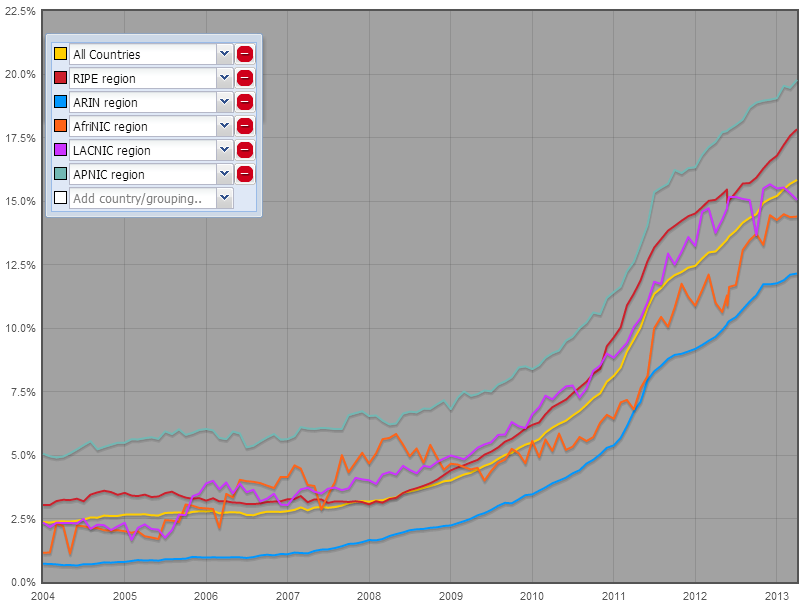
\includegraphics[width=0.4\textwidth]{img/v6-bgp-rirs.png}
\caption{Percentage of ASs that advertise an IPV6 prefix showing RIRs (source
\protect\cite{ripe_ncc_total_2013})}
\label{fig:bgp-rirs}
\end{figure}

It is also possible to combine the BGP routing data with the prefix allocation
data to work out how the delay between an organisation being allocated a prefix
and that prefix being advertised in the BGP routing tables. Karpilovsky et al.
find the average time for an allocated prefix to be advertised is 173 days, much
longer than the average of 52 days for IPv4 prefixes\cite{karpilovsky_quantifying_2009}.

An issue with using BGP tables for measuring IPv6 deployment is use of route
aggregation. Route aggregation is a feature of IPv6 designed to reduce the size of the
global routing table by advertising the largest possible prefix where a router
has routes to a number of consecutive prefixes. This means that a given prefix in
the BGP routing tables may refer to more than one AS, and in particular
connections at the edge of the internet are poorly represented in these
tables\cite{dhamdhere_measuring_2012}.


%\subsection{Usage Data \& Service Availability}
\subsection{User Measurements}

The first two methods explored look at data based on the
infrastructure of the internet. Another perspective can be a gained by analysing
data from the end users of the internet, whether that be individuals browsing
the web, organisations serving those web pages, or email servers sending mail
across the internet. Data concerning the usage and availability of services over
IPv6 on the internet whilst not strictly representing the deployment of IPv6 in
terms of the presence of the necessary infrastructure (although this
infrastructure must be
present) gives an insight into the deployment of IPv6 in terms of
how much the protocol is actually used rather than how widely it is supported.

The sources of data and the methods used in measurement of data from the users
and service providers of the internet generally fall into two categories:
enumerating and analysing the availability of services over IPv6 and measuring
how much these available services are being used. Availability data can be
collected by actively crawling the internet, whereas usage data is generally
collected via passive means such as Netflow\cite{shen_observations_2009} or by analysing server logs.

To gather data about the use of IPv6 by consumers, and the availability of IPv6
networking to end users, Colitti et al. at Google added code to the Google.com
website that tested IPv6 connectivity from browsers that connected to it. The
client code connected to both a dual-stack host and an IPv4 host to find out
whether IPv6 or IPv4 were preferred when both were available\cite{colitti_evaluating_2010}. Colitti et al.
find that between September 2008 and September 2009 IPv6 usage remains roughly
static between 0.2-0.25\%. Of further interest is how IPv6 is used when clients
use the protocol to connect, as their analysis shows that more of half of the IPv6 accesses
seen were conducted using the 6to4 tunnelling protocol. Another significant
possible usage of tunnelling is where Colitti et al. find that France has the
second highest working IPv6 ratio out of all countries surveyed, of which
almost all accesses were listed as of type "Native/tunnel/unknown". France is
the location of one of the single largest commercial deployment of IPv6
infrastructure, where the ISP Free has deployed 6rd\cite{rfc5569} to all of its
customers. This means that an even larger number of hosts than indicated are
using tunnelling methods rather than native IPv6, and more specifically 6to4 or
a variant thereof (6rd is a specialisation of 6to4 using an organisations
global IPv6 address space). Huston also presents some usage data in his 2008
article on IPv6 deployment, and similarly finds the amount of IPv6 traffic to
APNIC web servers to be around 0.2\% between 2004 and 2008\cite{huston_ipv6_2008}. Google's own data
collected since 2008 shows a significant uptake in the usage of IPv6, going from
the 0.2\% recorded in 2008 to 1.3\% as of May 2013, as shown in Figure
\ref{fig:google-access}. This is an increase of over
500\% in 5 years, which contrasts strongly against the static rate of IPv6 seen
in the previous 4 years. The usage of the 6to4 and Teredo tunnelling mechanisms
is also shown to have fallen to almost 0\% since 2008, although it is not
possible to tell how widely other tunnelling mechanisms such as 6rd are being
used.

\begin{figure}[htb]
\centering
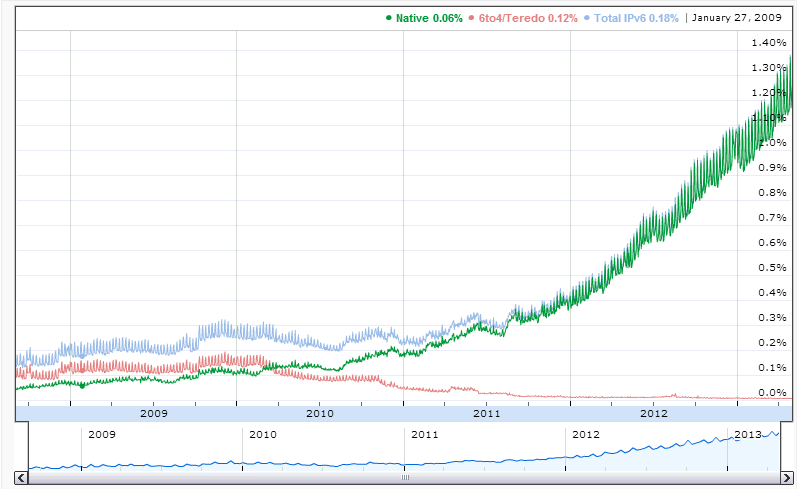
\includegraphics[width=0.4\textwidth]{img/v6-google-access.png}
\caption{Percentage of Users accessing Google using IPv6 between 2008 and 2013
(source \protect\cite{google_inc._statistics:_2013})}
\label{fig:google-access}
\end{figure}

Data detailing the availability of services over IPv6 can be used to get a
measure of how IPv6 is being deployed by the content and service producers and
providers of the internet. Widespread support of serving content and services
from IPv6 endpoints is a precursor to increased end-to-end deployment of IPv6
across the internet. The types of services that are surveyed for access over
IPv6 generally include web sites, email servers, and DNS servers
as the presence of these services can be easily remotely probed. Collecting data
on service availability is also easier than attempting to collect usage data
for a large sample size as availability data can be measured using active probes
that crawl a large number of sites.

Service availability data for web, email, DNS, NTP, Jabber, and email client
services over IPv6 is presented by Prior, who uses a colour coded scorecard
approach to indicate the availability of of these services at a number of
internet and research organisations, along with various technology companies and
government departments from around the world\cite{prior_ipv6_2012}. This testing is performed by
attempting to access the services related to the organisations over an IPv6
connection, using DNS records to derive addresses for all the services. An IPv4
connection is also made so it is possible to tell whether a service is only
provided over IPv4 or not at all. No historical data is provided, and the data
shown is refreshed periodically, but it is of interest to note the number of
research organisations and World IPv6 Day participants who do not provide
services over IPv6. A more extensive survey is presented by Crépin-Leblond at
ISOC England who has used the Alexa list of the top 1 million most accessed web
sites on the web\footnote[2]{http://www.alexa.com/topsites}
to create a web crawler that checks for IPv4 and IPv6 connectivity to services provided
at the domains of these sites.\cite{olivier_mj_crepin-leblond_ipv6_2010}. This
data is then linked to geographic data to present an indication of the progress
of the deployment of IPv6 on a country by country basis.
Historical data for the matrix is maintained, so it is possible to track service
availability from when data collection was started in 2010. Nikkhah et al. also
perform service availability using the Alexa lists but only checking for
web access, and find that whilst adoption of IPv6 has improved recently
performance problems exist due to a lack necessary support on the IPv6
backbone\cite{nikkhah_assessing_2011}.

Using availability data to measure the deployment of IPv6 is a promising
approach, allowing a fairly complete view across the web of services that
support IPv6 compared to usage data that is only available for specific sources,
and it gives a view of deployment that is closer to actual use than the data for
prefix allocation and BGP route announcement provides. However, this method of
collecting data is relatively recent so historical records do not stretch as far
back as those for the other methods and little published
analysis has been performed on the data.

\subsection{Distributed Active Measurement}

As an extension to user measurements, it is possible to collect measurements by
deploying a distributed network of probes around the world to
gather data from many different parts of the internet. The CAIDA
Archipelago (Ark)
project has deployed over 70 probes to locations around the world, with 30 of these
having an IPv6 connection\cite{caida_archipelago_2013}. The Ark project performs active scanning of every
IPv6 prefix announced in the BGP routing tables, and uses this data to map the
topology of the internet. Another distributed monitoring system with a
larger number of probes is the RIPE Atlas project, with nearly 3000 active
probes, of which over 800 are IPv6 enabled\cite{ripe_ncc_ripe_2013}. The Atlas probes engage in
significantly fewer measurements as many are deployed on domestic
broadband connections by volunteers and perform ping, traceroute and DNS
queries to a small number of predefined servers, including a number of the DNS
root servers. Both projects offer embedded hardware probes to the community as a
means to increase coverage.

Musulin and Duisters use a small sample of RIPE Atlas data collected over 9 days
in 2011 to explore the comparison between IPv6 and IPv4 measurements performed
by the Atlas nodes\cite{musulin_analysis_2011}. They find that the reliability and performance of IPv6 is
lower than IPv4, although also state that it was not possible to eliminate all
tunnelled traffic from the IPv6 measurements, a factor that will affect the
performance and stability of measurements due to the added complexity of
tunnelled connections. 

Measurements from distributed monitoring systems can provide a view of the
internet from a large number of vantage points, but have the drawback of
requiring significant investment and overhead to produce and distribute
monitoring probes. This means that only a small number of projects
have managed to achieve significant distribution of monitoring nodes. The
RIPE Atlas project have made it possible for researchers to perform their own
studies using the entire network of probes by allowing Use Defined Measurements
(UDMs) that are run on many probes\cite{ripe_ncc_user-defined_????}, hence making distributed active
measurement a viable option for further studies of IPv6.





